\chapter{Introduction}\label{chap:intro}

\section{PFAS}
\textit{Per}- and polyfluorinated alkyl substances (PFAS) are a large group of synthetic compounds that are used in numerous industrial and consumer products. As a result of decades of use, PFAS are ubiquitous in soils, groundwater, and surface water \citep{rankin2016north}. PFAS are both oil and water repellent, which makes them ideal as foaming agents and flame retardants, as a coating for the famous waterproof Gore-Tex\textsuperscript{\textregistered} textiles and non-stick, frictionless Teflon\textsuperscript{\texttrademark} cookware \citep{du2014adsorption}. Despite having many desirable properties, widespread production and distribution of PFAS with waterways has led to accumulation in soil, crops, wildlife, and higher trophic levels, including humans \citep{bhhatarai2011,Lau2007}. The synthetic structure of PFAS and the strength of the C-F bonds makes these chemicals resistant to natural degradation \citep{krafft2015per}, and although the mechanisms of PFAS toxicity are not well understood, they are also suspected to be bioaccumulative and toxic \citep{ding2013physicochemical,Lau2007}. Today, PFAS are recognized as emerging persistent organic pollutants (POPs) \citep{ECHA2020}, and legislation has been introduced to regulate the manufacture, sale, and use of several PFASs \citep{EPA2014,EC2020PFAS,goldenman2017study}. Two of the most widely used and distributed compounds, PFOA and PFOS, are listed under the Stockholm Convention as POPs. Considerations to add other PFAS compounds to this convention are ongoing \citep{EC2020PFAS}. An important example is efforts by the German Environment Agency to identify a new class of compounds called PMT (persistent, mobile, and toxic) and vPvM (very persistent, very mobile) under REACH, the EU chemicals regulation (Registration, Evaluation, Authorization and Restriction of Chemicals) and ECHA (the European Chemicals Agency) \citep{hale2020persistent}. PMT/vPvM substances have properties that are not covered by the Stockholm Convention, but are an equally great threat to the environment and maintaining the purity of the world's drinking water resources. A great deal of research has been done to develop ways of effectively remediating PFAS-contaminated soil and water. One of these is the overarching focus of this thesis. 

\subsection{Overarching research project}
A great deal of research has been done to develop ways of effectively remediating PFAS-contaminated soil and water. One of these is the overarching focus of this thesis. The aim of this work has been to study whether biochar from various lightly contaminated organic waste materials can be used as a sorbent in the remediation of PFAS-contaminated soil and water. A sorbent is a porous, carbonaceous material with the ability to remove contamination from water by strong binding to its internal structure. Remediation work by the use of a sorbent is done by mixing the sorbent with the contaminated water or soil \textit{in situ}, eliminating transportation needs of the contaminated masses.  

\subsection{PFAS in industrial runoff and wastewater}
The sources of PFAS contamination are typically local industrial point sources such as paper mills \citep{lee2020legacy,langberg2021paper}, leaching from landfills \citep{masoner2020landfill}, firefighting training facilities \citep{filipovic2015historical}, and discharge from fluorochemical plants \citep{gebbink2017presence} into the wastewater. This puts wastewater treatment plants (WWTPs) under additional pressure  to adequately treat wastewater so as to avoid further release of PFAS chemicals into the environment  \citep{Morin2017flameWaste}. By restricting many long-chain PFASs, new challenges related to controlling the spread and effects of increased use of short-chain replacements have emerged \citep{knutsen2019leachate}. Short-chain PFAS have higher mobility and tend to slip through existing water treatment processes, thereby contaminating food and drinking water \citep{hale2020persistent,brendel2018short}. Although short-chain PFAS are less bioaccumulative, persistence and toxicity are expected to be equivalent to the substances they replace \citep{EC2020PFAS}. 

\subsection{Physicochemical and sorption properties}\label{sec:physchem} 
PFAS are synthetic organic compounds that consist of a polar head, most commonly a carboxyl or sulfate functional group, and a non-polar chain of alkyl moieties that are either fully substituted (per-), or partly substituted (poly-), with fluorine \citep{wang2011physchem}. PFASs are divided into compound classes based on functional group and degree of fluorination, of which perfluorinated carboxylic acids (PFCAs) and perfluorinated sulfonic acids (PFSAs) are the most common. Since fluorine is the most electronegative atom identified, the C-F covalent bonds make one of the strongest known bonds in organic chemistry (BDE=485 kJ mol\textsuperscript{-1}) \citep{Lau2007}. The nature of these bonds become significant for two main reasons: 1) C-F bonds are not found naturally in the environment, and this means that no natural enzymes can degrade them. This accounts for why PFAS is persistent in the environment \citep{hale2020persistent,krafft2015per}. 2) The chain of repeating CF\textsubscript{2} units consists of highly polar bonds with a symmetric structure. This causes the entire surface area of the PFAS tail to carry a net negative charge. This in turn minimizes the ability of PFAS to undergo either van der Waals interactions with other molecules or hydrogen bonds due to the lack of a positive dipole \citep{Arp2006}. The combined properties of low van der Waals and non-polarity make the tail neither hydrophobic nor lipophobic. The result is a new compound class that is "everything-phobic". This everythingphobic-ness causes \acrshort{PFAS} to behave uniquely in the environment by being more mobile than other organic pollutants that often are hydrophobic \citep{hale2020persistent}. A more detailed discussion on the mobility of PFAS is given in the following section.  

The behavior of PFAS is often discussed interchangeably with hydrophobic compounds that have strong affinities to hydrophobic surfaces. More correctly, sorption of PFAS should be discussed in terms of a shear pushing of PFAS by water molecules onto hydrophobic surfaces \citep{Arp2006}. The cavity formation energy barrier rises for every $CF_2$ moiety present, making dissolution increasingly difficult at longer chain lengths \citep{bhhatarai2011,Arp2006}. This is the primary mechanism that reduces the mobility of PFAS leading to accumulation in soils and biota. The effect of chain length on partitioning between dissolved and solid phases is one of the main topics that will be discussed in further detail throughout this thesis.

Sorption is a collective term used to describe removal of molecules from the water phase by \textit{ab}sorption (dissolution-like partitioning into a material) and \textit{ad}sorption (bonding on the surface of a solid). The role van der Waals forces play, as well as other mechanisms of attraction and repulsion for PFAS interaction with sorbents, will be discussed in a later section on sorption mechanisms \cref{sec:mechanisms}. 

In contrast to the everything-phobic chain, the hydrophilic head of PFAS can hydrogen bond to other polar compounds such as water, and interact electrostatically with positively charged species \citep{sigmund2022sorption}. Since the head groups of PFAS are acids, knowledge of its protonation state is key to further understand solubility and volatility, which in turn affect the mobility and long range transport potential of these chemicals. Determining the acid dissociation constants (\(pK_a\)) of PFAS has been the subject of much debate in the scientific community \citep{Goss2009comment}. This debate is linked to the complexity of how PFAS behaves at different concentrations, and on the water surface. However, most researchers agree that \(pK_a\) values are below 1 and decrease with increasing chain length \citep{wang2011physchem,Reemtsma2016}. Thus, PFAS are expected to be negatively charged at environmentally relevant pH levels, enhancing their ability to dissolve in water by charge-assisted H-bonds \citep{Reemtsma2016}. For example, PFOA has a water solubility of 3.4 g L\textsuperscript{-1} \citep{PFOA}, whereas its structural analog, perfluorooctane (PFO) \citep{PFO}, which has no polar functional group, exhibits a far lower solubility (1 mg/L). Furthermore, hydrophobic organic compounds (HOCs) are are much more insoluble, for example hexachlorobenzene (HCB) has a solubility of $0.005 mg/L$ \citep{mcphedran2013hydrophobic}. 

\subsection{Mobility and accumulation of PFAS in the environment}
The combination of an everything-phobic tail and an ionizable hydrophilic head makes understanding the mobility of PFAS in the environment more complex than that of legacy POPs \citep{cabrerizo2018legacy,Arp2006}. Since PFASs are not very volatile---low vapor pressure and air-water partition coefficient ($K_{AW}$)---aqueous solubility and uptake in migrating biota play the primary roles for the mobility of PFAS in the environment \citep{Arp2006}. \cite{Schlabach2017} reported that a diverse suite of PFASs are present in Arctic biota such as fish, polar bears and mink. Sorption mechanisms are also slightly different for PFAS compared to hydrophobic and lipophilic legacy POPs like polychlorinated biphenyls (PCBs), hexacholorocyclohexanes (HCHs), and polycyclic aromatic hydrocarbons (PAHs), which have higher volatility, lower solubility and higher lipophilicity \citep{cabrerizo2018legacy,Cornelissen2005,li2018}. The latter property is often expressed as the octanol water partition coefficient (\(K_{OW} = C_{o}/C_w\)). This coefficient is used to represent partitioning between a hydrophobic phase represented by octanol (numerator) and the aqueous phase (denominator) \citep{Reemtsma2016}. The lower \(K_{OW}\) of PFAS compared to HOCs can be used to explain why PFAS more readily leaches from soils to groundwater \citep{Cornelissen2005,du2014adsorption}). A more environmentally relevant parameter than \(K_{OW}\) is \(K_{OC}\), the organic carbon-water partition coefficient. \(K_{OC}\) is an important driver of the sorption of PFAS in soils and sediments \citep{zareitalabad2013perfluorooctanoic}. This coefficient also represents the higher tendency of PFAS to leach from soils to groundwater, as compared to compounds with higher $K_{OC}$ like PAHs and PCBs that sorb more strongly to organic matter \citep{Cornelissen2005}. 

%%%%%%%%%%%%%%%%%%%%%%%%%%%%%%%%%%%%%%%%%%%%%%%%%%%%%%%%%%%%%%%%%%%%%%%%%%%%%%%%%%%%%%%%%%%%%%%%%%%%%%%%%%%%%%%%%%%%%%%%%%%%%%%%%%%%%%%%%%%%%%%%%%%%%%%%%%%%%%%%%%%%%%%%%%%%%%%%%%%%%%%%%%%%%%%%%%%%%%

\section{Biochar---from traditional soil amendment to sorbents for emerging contaminants}
Biochar is a common term for the carbon-enriched product produced from pyrolysis of biomass \citep{LehmannAndJoseph2015}. Common feedstocks used to produce biochar are various crop residue, poultry litter, wood shavings, and grain straws \citep{Ahmad2014}. Pyrolysis is a thermal treatment method that burns organic matter in the absence of oxygen, a process which forms fused aromatic ring structures that have high porosity and surface area and low residual functional groups \citep{LehmannAndJoseph2015}. Biochar improves soil health by increasing water retention and carbon content, increasing pH of acidic soils, and securing a more steady nutrient release \citep{das2020application}. In addition, the ash co-products enrich biochar with macro- and micro nutrients that are also beneficial in agriculture. The use of biochar as a soil amendment dates back 2,500 years to the pre-Columbian Amazonian peoples \citep{Tindall2017}. They used slash-and-char techniques to produce biochar which they spread over their fields. The result was \textit{terra preta}, the most fertile soil known \citep{Ahmad2014}. Today, biochar has numerous multidisciplinary applications, such as soil fertility improvement, waste recycling, carbon sequestration, and sorbents for remediation of contaminated sites \citep{beesley2011review}.

\subsection{Biochar as sorbents}
The application of biochar as a sorbent for soil and water remediation, is relatively new \citep{beesley2011review}. Historically, activated carbon (AC) from fossil coal sources, has been used for soil remediation exclusively \citep{hagemann2018activated}. The term "activation" is used to describe the process of thermal treatment ($<$ 800\textdegree C) of a carbonaceous material by steam ($\mathrm{H_2O}$) or carbon dioxide ($\mathrm{CO_2}$) that expands its surface area by creating new nanopores ($<$2nm), thereby increasing sorption capacity \citep{LehmannAndJoseph2015}. Simultaneously, surface functional groups are oxidized to create a smoother, aromatic surface that improves sorption affinity to organic molecules \citep{sajjadi2019comprehensive}. This process improves the sorptive affinity of the biochar, making it an ideal sorbent for organic pollutants \citep{Ahmad2014}. Current challenges connected to production of AC include high operating costs and energy inputs, the use of non-renewable fossil fuel coal as raw material \citep{Li2019}, and the fact that the activation process is associated with higher carbon losses and lower yields, resulting in less carbon sequestration \citep{Sormo2021}. Biochar is often termed a universal sorbent because its surface will both have regions of hydrophilic or charged functional groups that are ideal for electrostatically binding cationic organic and inorganic species such as heavy metals \citep{silvani2019can,zhang2013sorption}, and other regions of more condensed, aromatic surfaces that are better suited to sorb hydrophobic molecules \citep{Cornelissen2005}.

Researchers have had several successful attempts at using activation technology on biochar instead of fossil coal as sorbents for organic contaminants \citep{Sormo2021}. Commercial production is growing internationally and activated biochar is now widely used for soil remediation \citep{hagemann2018activated}. In recent years, there has been much interest in studying whether also non-activated biochars can be effective sorbents for use in contaminant remediation and water purification \citep{hagemann2018activated}. The main advantages of using biochar instead of AC are the potential for carbon sequestration \citep{smith2016soil} and reduced reliance on Chinese coal mines \citep{zheng2019influence}. If engineered correctly, biochar is expected to be at least as effective as AC in sorption of organic pollutants \citep{Sormo2021}. Important aspects have been to study how feedstock, pyrolysis temperature and residence time affect biochar properties \citep{Hale2016}. Since feedstocks used to produce biochars often have a heterogeneous composition of elements other than carbon, they need to be pyrolyzed at higher temperatures to gain a sufficient surface area and porosity for sorption \citep{beesley2011review}. By adjusting pyrolysis temperature, biochar can be tailored to match the physicochemical properties of the contaminants of interest \citep{Hale2016}. The oxygen to carbon (O/C) ratio is used as proxy for polarity and hydrophobicity of a sorbent's surface, where a high ratio is indicative of a more oxidized surface high in oxygen-containing functional groups. Likewise, the hydrogen/carbon (H/C) ratio is used as proxy for aromaticity, where a lower ratio is indicative of a higher degree of fused aromatic ring structures that form a more porous biochar material \citep{Ahmad2014}. The O/C and H/C ratios have been found to decrease with increasing pyrolysis temperature \citep{Hale2016}. Therefore, biochars produced at high temperatures (700-900 \textdegree C) are the most suitable for sorbing organic contaminants \citep{Figueiredo2018}. 

One of the main challenges proposed by the application of non-activated biochar in natural systems is its lower porosity than AC \citep{leng2021overview}. High porosity becomes particularly important when carbonaceous sorbents are applied to organic matter (OM)-rich soils because small pores are vulnerable to pore blockage by large organic molecules \citep{Sorengard2019}. However, application of biochar to soil with low OM content has proved to be equally effective as the use of non-activated biochar \citep{Alhashimi2017}. This way, biochar provides a contribution to reduce the demand for AC in remediation, which in the future may only be limited to OM-rich soils and ultra-fine water cleansing. The latest research on biochar has been to study the potential for producing biochar sorbents from various lightly contaminated organic waste materials such as papermill waste \citep{van2010effects}, sewage sludge \citep{fathianpour2018lead}, biosolids \citep{wang2011}, and palm oil mill sludge \citep{lam2017adsorption} with an end goal to achieve a net negative GWP and energy use and a better waste handling alternative to landfilling or incineration \citep{Alhashimi2017}. Ongoing research, including the present work, investigates the effectiveness of non-activated biochar as sorbents from waste feedstocks for PFAS. 

\subsection{Sorption mechanisms}\label{sec:mechanisms}
Sorption to BC involves several factors such as biochar morphology, contaminant concentration, competing contaminants, sorbate physicochemical properties, and molecular size \citep{Li2019,du2014adsorption}. Sorption to porous carbonaceous materials occurs via chemisorption (covalent sorbent-sorbate bonding), and physisorption (encapsulation of the adsorbent in the biochar's maze of pores and electrostatic attraction) \citep{Li2019}. Researchers have postulated that sorption of PFAS occurs primarily via direct (specific) polar interactions, hydrophobic (non-specific) interactions, and ion exchange mechanisms \citep{Hale2017fire,yu2009sorption}. Polar interactions include H-bond and charge-assisted H-bond interactions. Non-specific hydrophobic interactions can more accurately be described as high cavity formation energy which results from the sum of forces that limit solubility of large, non-polar molecules in water \citep{Arp2006,sigmund2022sorption}. Electrostatic interactions involve both attraction and repulsion. Cation bridging is one form of electrostatic attraction. Determination of sorption isotherms is a central part to understanding the interactions between biochar and PFAS and sorption capacity \citep{yu2009sorption,Li2019}.

%%%%%%%%%%%%%%%%%%%%%%%%%%%%%%%%%%%%%%%%%%%%%%%%%%%%%%%%%%%%%%%%%%%%%%%%%%%%%%%%%%%%%%%%%%%%%%%%%%%%%%%%%%%%%%%%%%%%%%%%%%%%%%%%%%%%%%%%%%%%%%%%%%%%%%%%%%%%%%%%%%%%%%%%%%%%%%%%%%%%%%%%%%%%%%%%%%%%%%%%%%%%%%%%%%%%%%%%%%%%%%%%%%%%%%%%%%%%%%%%%%%%%%%%%%%%%%%%%%%%%%%%%%%%%%%%%%%%%%%%%%%%%%%%%%%%%%%%%%%%%%%%%%%%%%%%%%%%%%%%%%%%%%%%%%%%%%%%%%%%%%%%%%%%%%%%%%%%%%%%

\section{Valorization of sewage sludge}
Recycling and valorization of waste have become key areas of interest in research and development aimed at achieving a transition to a more circular economy \citep{Ahmad2014}. In recent years, the European Union has invested substantial funding in projects that work on developing remedial techniques for the treatment of soil and water contaminated with PFAS (see \cref{sec:SDGs}) \citep{EC2020PFAS,ECHA2020}. One of the most promising techniques developed so far is an \textit{in situ} treatment that involves applying sorbents which immobilize PFAS from the bioavailable aqueous phase by strong sorption to biochar \citep{Ahmad2014,Sormo2021,Kupryianchyk2016b}. \cref{fig:cornelissen_sorption} describes...

\begin{figure}
    \centering
    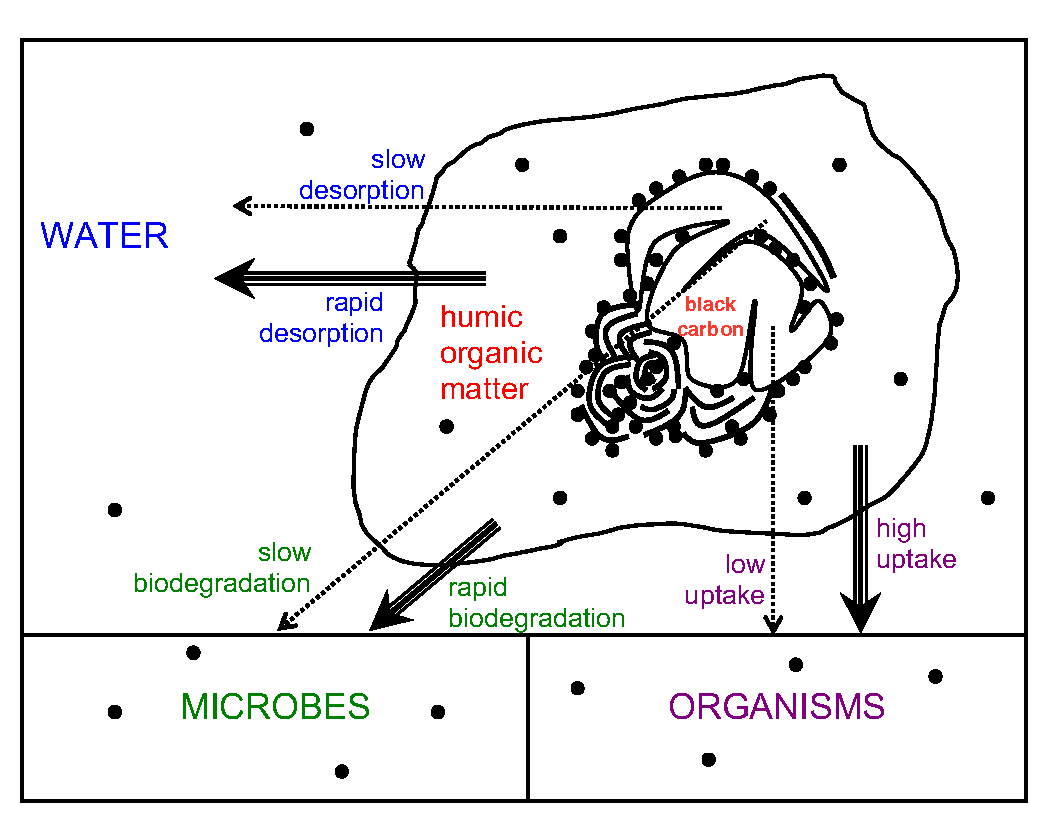
\includegraphics[width=\textwidth]{Diagrams/Cornelissen_sorption.pdf}
    \caption{Sketch adapted from \citep{Cornelissen2005} of the differences in sorption The dots represent organic molecules , }
    \label{fig:cornelissen_sorption}
\end{figure}

\subsection{Sewage sludge biochar as sorbent for PFAS}
Biosolids are the residual semi-solid material waste left over from wastewater treatment. They are produced in large quantities and are expensive to dispose of because they are often polluted with heavy metals, micro plastics and organic pollutants \citep{Raheem2018}. High moisture and ash contents, as well as the presence of heavy metals and a cocktail of organic contaminants contained in sewage sludge, make treatment and disposal difficult \citep{Li2019}. Incineration or landfilling, disposal methods often resorted to, release significant greenhouse gases (GHG), fly ash and PAHs \citep{huang2022comparative}. These disposal methods are associated with increased risk that contaminants leach into soils and groundwater \citep{propp2021organic}. 

Wastewater treatment plants (WWTPs) have started to look at possible ways to handle biosolids and raw sewage sludge in a more sustainable and cost-effective manner \citep{Raheem2018}. One is to generate energy from waste. With the help of microorganisms, it is possible to produce digestate, the liquid residual fraction from the anaerobic treatment of sewage sludge and other organic wastes  (AD) (\cref{eq:AD}). This digestate is now being used for the commercial production of bio gas. In some cases, biosolids are applied to agricultural fields as fertilizers \citep{moodie2021legacy}. However, high contents of micro and macro plastics, and heavy metals, may limit the use of biosolids in agriculture \citep{mohajerani2020microplastics}.

Research into the production of biochar using digestate and raw sewage sludge as feedstocks, represents a promising novel strategy to find sustainable ways to valorize organic waste. Production of biochar is particularly attractive because it is considered one of the most promising carbon sequestration technologies that also transforms a problematic waste material into an economically valuable resource \citep{arvaniti2014sorption}. A higher content of inorganic ions, reflected in a higher ash content, means that sewage sludge has a higher yield than cleaner, wood-based feedstocks \citep{Cantrell2012}. One of the clear benefits associated with the presence of more ash is a lower loss of volatile carbon because inorganic ions raise the bond dissociation energy of organic and inorganic carbon \citep{Cantrell2012,Enders2012}. 

Still today, industrial production of sorbents by pyrolysis of sewage sludge is still in a pioneering phase. Some of the challenges include: 1) Sewage sludge biochar has a lower carbon content than more homogeneous, wood-based feedstocks. It likely has a low surface area and porosity, and hence, poor sorption strength. Due to its lower porosity, it is expected that uptake may be lower than by AC. In order to achieve an acceptable quality of treatment for contaminated soil and water. A higher dosage of biochar, or more frequent biochar filter exchange, are needed. 2) Non-activated biochar possesses of more oxygen and nitrogen-containing functional groups, making it more polar. This in turn results in it being able to attract charged and polar contaminants to a greater extent. Non-activated biochar contains a higher non-carbonized fraction that interacts with contaminants in a different way than fully condensed, aromatic structures. One of the main focuses of this thesis is discussing the relevance and benefits of this more heterogeneous matrix for sorption of PFAS. 3) Due to the heterogeneity of sewage sludge, biochar will vary in composition. The result is that biochar, from time to time, will exhibit inconsistent sorption capacities. 4) Bio oils and syn-gas are by-products from the production of biochar. They are expected to contain organic pollutants, and constitute a possible source of greenhouse gases, particulate matter, and heavy metals. Pollution control measurements were conducted simultaneously by research partners. These will provide important information relevant for an overall life cycle assessment (LCA) of biochar, a theme that will be further discussed in \cref{sec:LCA}). 
